In this section, we present an experimental evaluation of our
  language.  The examples provided highlight two main points: firstly,
  the representation using choreographic language is significantly
  more concise; secondly, we demonstrate that PRISM behaves similarly
  on both the projection and the original model in PRISM also in our
  implementation.
%In order to show that using choreographies is beneficial in the
%presence of concurrency, we included an example modelling a single
%process.
 % We have decided to provide two examples with concurrency and one
% without .  
In particular, we focus on six benchmarks: a modified version of the
example reported in Section \ref{sec:example}; a simple Peer-To-Peer protocol;  the Bitcoin Proof of Work
protocol~\cite{DBLP:journals/concurrency/BistarelliNGLMV23}; the
Hybrid Casper
protocol~\cite{DBLP:journals/distribledger/GallettaLMV23}; a synchronous leader election protocol~\cite{IR90} and a modelization of the dining cryptographers~\cite{Cha88}.  The
generated PRISM files can be found in our online repository
\cite{repository}.


\mypar{A Modified thinkteam Protocol.}
In this modified version of the thinkteam protocol introduced in the earlier sections, we extend the protocol to involve generalised interactions with possible many receivers. Specifically, the \texttt{CheckOut} process now communicates with two users simultaneously, \texttt{User1} and \texttt{User2} each tasked with performing distinct actions upon access to the file. 

 In the first branch, \texttt{User1} increments the variable \texttt{x} by 1, while \texttt{User2} decrements the variable \texttt{y} by 1. Conversely, in the second branch, the roles are reversed, with \texttt{User1} decrementing \texttt{x} and \texttt{User2} incrementing \texttt{y}.

 \begin{lstlisting}[style=chor-color,breaklines=true, postbreak=\mbox{\textcolor{red}{$\hookrightarrow$}\space},caption={Choreography for the Modified thinkteam Protocol},captionpos=b,label={ex1-chor}]
   C0 := CheckOut $\rightarrow$ User1, User2 : (+["1*lambda"] " " "(x=x+1)"  "(y=y-1)"; C1
                                       	+["1*lambda"]  " " "(x=x-1)"  "(y=y+1)";  C2)
   C1 :=  CheckOut $\rightarrow$ User1, User2 : (+["1*theta"] ; C0)  
   C2 :=  CheckOut $\rightarrow$ User1, User2 : (+["1*mu "] ; C1   +["1*mu "] ;  C2)
 \end{lstlisting}

 Part of the generated PRISM model is reported in Listing \ref{ex1-gen}. 

 \begin{lstlisting}[style=prism-color,caption={Generated PRISM program},captionpos=b,label={ex1-gen}]
   module CheckOut
      CheckOut_STATE : [0..2] init 0;
      [MMHOL]  (CheckOut_STATE=0) -> 1 :  (CheckOut_STATE'=1);
      [FFSFW]  (CheckOut_STATE=0) -> 1 :  (CheckOut_STATE'=2);
      [ULCFN]  (CheckOut_STATE=1) -> 1 : (CheckOut_STATE'=0);
      [YHHWG]  (CheckOut_STATE=2) -> 1 : (CheckOut_STATE'=1);
      [XWSAO]  (CheckOut_STATE=2) -> 1 : (CheckOut_STATE'=2);
   endmodule
$\ldots$
   module User2
      User2_STATE : [0..2] init 0;
      [MMHOL]  (User2_STATE=0) -> lambda : (y'=y-1)&(User2_STATE'=1);
      [FFSFW]  (User2_STATE=0) -> lambda : (y'=y+1)&(User2_STATE'=2);
      [ULCFN]  (User2_STATE=1) -> mu : (User2_STATE'=0);
      [YHHWG]  (User2_STATE=2) -> theta : (User2_STATE'=1);
      [XWSAO]  (User2_STATE=2) -> theta : (User2_STATE'=2);
endmodule
\end{lstlisting}
The generated PRISM model appears less clear compared to its
choreographic representation, primarily due to its lack of sequential
structure and lower readability.  In the PRISM model, the absence of a
clear sequential structure makes it harder to follow the flow of
interactions between components, 
since module definitions and transition labels can be more challenging
to read and comprehend compared to the concise and structured nature
of the choreographic language.



\mypar{Simple Peer-To-Peer Protocol}
This case study describes a simple peer-to-peer protocol based on BitTorrent\footnote{\url{https://www.prismmodelchecker.org/casestudies/peer2peer.php}}. The model comprises a set of clients trying to download a file that has been partitioned into $K$ blocks. Initially, there is one client that has already obtained all of the blocks and $N$ additional clients with no blocks. Each client can download a block from any of the others but they can only attempt four concurrent downloads for each block.\\
The code we analyze with $K=5$ and $N=4$ is reported in Listing \ref{ex2-code}.
\begin{lstlisting}[style=chor-color,caption={Choreography for the Peer-To-Peer Protocol},captionpos=b,label={ex2-code}]
{
PeerToPeer := Client[i] $\rightarrow$ Client[i]: 
			(+["rate1*1"]  "(b[i]1'=1)"$\&\&$" " . PeerToPeer
			 +["rate2*1"]  "(b[i]2'=1)"$\&\&$" " . PeerToPeer
			 +["rate3*1"]  "(b[i]3'=1)"$\&\&$" " . PeerToPeer
			 +["rate4*1"]  "(b[i]4'=1)"$\&\&$" " . PeerToPeer
			 +["rate5*1"]  "(b[i]5'=1)"$\&\&$" " . PeerToPeer)
}
\end{lstlisting} 

Part of the generated PRISM code is shown in Listing \ref{ex2-gen} and it is faithful with what is reported in the PRISM documentation. 
\begin{lstlisting}[style=prism-color,caption={Generated PRISM program for the Peer-To-Peer Protocol},captionpos=b,label={ex2-gen}]
module Client1
	Client1 : [0..1] init 0;
	b11 : [0..1]; 
	b12 : [0..1]; 
	b13 : [0..1]; 
	b14 : [0..1]; 
	b15 : [0..1]; 

	[] (Client1=0)  $\rightarrow$ rate1 : (b11'=1)$\&$(Client1'=0); 
	[] (Client1=0)  $\rightarrow$ rate2 : (b12'=1)$\&$(Client1'=0); 
	[] (Client1=0)  $\rightarrow$ rate3 : (b13'=1)$\&$(Client1'=0); 
	[] (Client1=0)  $\rightarrow$ rate4 : (b14'=1)$\&$(Client1'=0); 
	[] (Client1=0)  $\rightarrow$ rate5 : (b15'=1)$\&$(Client1'=0); 
endmodule
\end{lstlisting}
\begin{figure}[h]
   \centering
   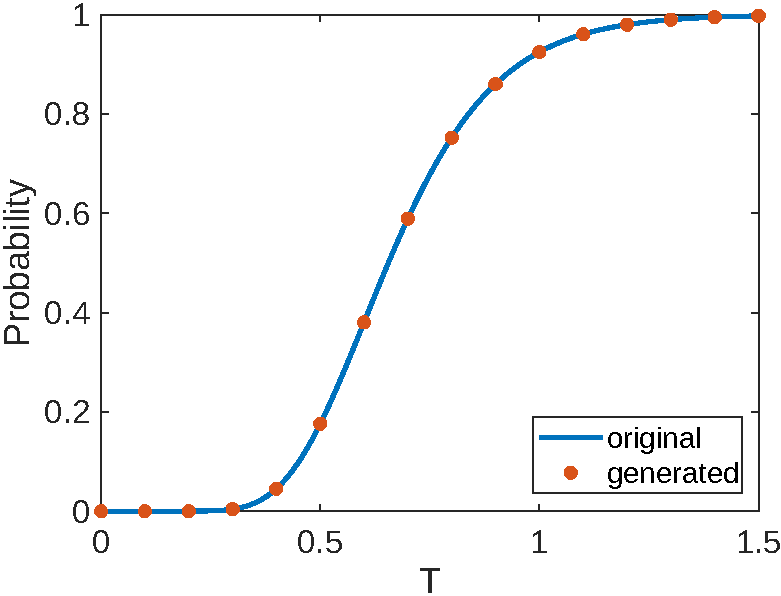
\includegraphics[scale=0.35]{peertopeer.pdf}	
   \caption{Probability that clients received all the block before $T$, with $0\leq T \leq 1.5$}
   \label{ex2-res}
   \end{figure}
   
   In Figure \ref{ex2-res}, we compare the probabilities that all clients (in a model with 4 
   clients: \codeprism{Client1}, $\ldots$, \codeprism{Client4}) have received all blocks 
   within the time interval $0 \leq T \leq 1.5$, as obtained from both our generated model 
   and the model reported in the documentation. This property serves as a benchmark to 
   evaluate whether the generated model preserves the expected behavior of the original 
   specification. In this case, there are no differences in the results or the time required 
   to compute the property.

\mypar{Proof of Work Bitcoin Protocol.}
In \cite{DBLP:journals/concurrency/BistarelliNGLMV23}, the authors extended the PRISM model checker syntax to incorporate dynamic data types, enhancing its capabilities to model the Proof of Work protocol used in the Bitcoin blockchain \cite{bitcoin}. 

In summary, the code depicts miners engaging in
  solving PoW, updating their ledgers, and communicating with the
  network.  The indices $i$ represent the module renaming feature of
  the choreographic language. Thus, each interaction will be repeated
  for each miner and hasher of the protocol that we are
  considering. The protocol works as follows. 
  \begin{lstlisting}[style=chor-color,breaklines=true, postbreak=\mbox{\textcolor{red}{$\hookrightarrow$}\space},caption={Choreography for the Proof of Work Bitcoin Protocol},captionpos=b,label={ex3-code}]
   {
   PoW $\coloneqq$ Hasher[i] $\rightarrow$ Miner[i] :
   (+["mR*hR[i]"]  " " "(b[i]'=createB(b[i],B[i],c[i]))&(c[i]'=c[i]+1)" ; 
      Miner[i] $\rightarrow$ Network : (["rB*1"] "(B[i]'=addBlock(B[i],b[i]))" 
                                       foreach(k!=i) "(set[k]'=addBlockSet(set[k],b[i]))"@Network;PoW)
    +["lR*hR[i]"] ; 
      if "!isEmpty(set[i])"@Miner[i] then { 
         ["r"] "(b[i]'=extractBlock(set[i]))"@Miner[i] ;  
            Miner[i] $\rightarrow$ Network : (["1*1"] "(setMiner[i]'=addBlockSet(setMiner[i],b[i]))" 
                                                "(set[i]' = removeBlock(set[i],b[i]))";PoW) 
      }
      else{
         if "canBeInserted(B[i],b[i])"@Miner[i] then { 
            ["1"] "(B[i]'=addBlock(B[i],b[i]))&(setMiner[i]'=removeBlock(setMiner[i],b[i]))"@Miner[i];
            PoW 
         }
         else{PoW}
      }
   )
   } 
   \end{lstlisting}
  When synchronising with
  the hasher, a miner tries to solve a cryptographic
  puzzle. Successful attempts add a new block to its ledger and update other miners' block sets. Unsuccessful attempts involve extracting a block, updating its ledger and block sets, and continuing the PoW process.
  \begin{figure}[h]
   \centering
   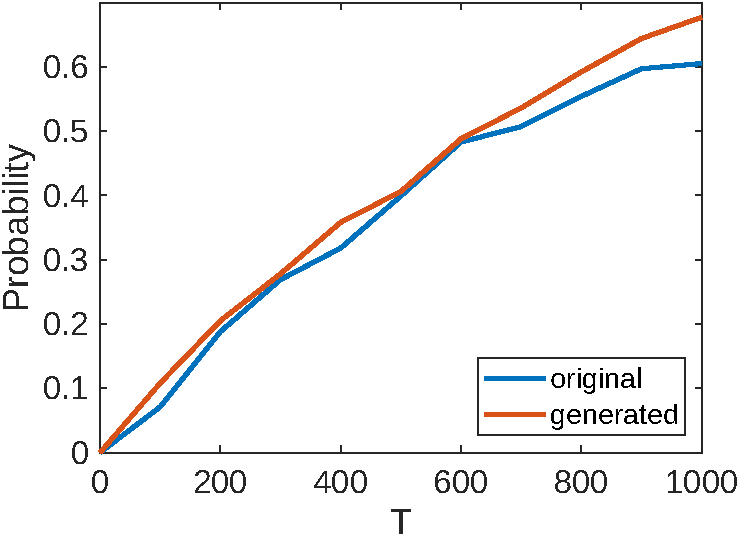
\includegraphics[scale=0.35]{example.pdf}	
   \caption{Probability that a block is created within $T$ time units, $0\leq T\leq 1000$}
   \label{ex3-res}
\end{figure}
The PRISM model we created is more verbose than the one in \cite{DBLP:journals/concurrency/BistarelliNGLMV23}, mainly because we consistently generate the else branch for if-then-else expressions, resulting in a higher number of instructions. Despite this, the experimental results for block creation probability within a bound time $T$ (Figure \ref{ex3-res}) remain unaffected. Any discrepancies between the original and generated models are due to inherent variations in the simulation-based calculation of probability.


\mypar{Hybrid Casper Protocol.}
\begin{comment}
\begin{wrapfigure}[12]{l}{4.5cm}
	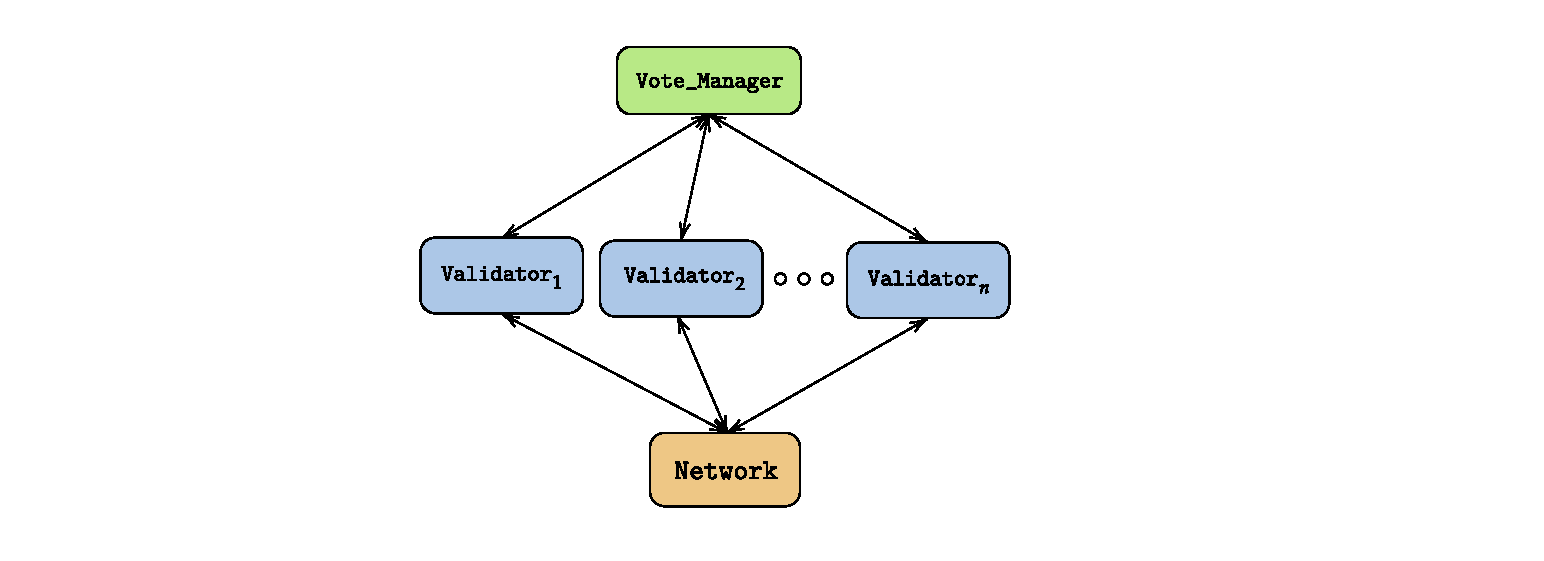
\includegraphics[scale=0.45]{ethereum.pdf}	
\end{wrapfigure} 
\end{comment}
We now present the Hybrid Casper Protocol \cite{DBLP:journals/distribledger/GallettaLMV23}. The Hybrid Casper protocol represents a hybrid consensus protocol for blockchains, merging features from both Proof of Work and Proof of Stake protocols. 
\begin{lstlisting}[style=chor-color,tabsize=2,breaklines=true, postbreak=\mbox{\textcolor{red}{$\hookrightarrow$}\space},	caption={Excerpt of the Hybrid Casper Protocol as a choreography},captionpos=b,label={ex5-code}]
{
PoS := Hasher[i] -> Validator[i] :
(+["mR*1"]  "(b[i]'=createB(b[i],L[i],c[i]))&(c[i]'=c[i]+1)"; 
	if "!(mod(getHeight(b[i]),EpochSize)=0)"@Validator[i] then{$\ldots$}
	else{
		Validator[i] -> Vote_Manager :(["1*1"]  "(Votes'=addVote(Votes,b[i],stake[i]))"; PoS)
	}
 +["hR*1"]  ; if "!isEmpty(set[i])"@Validator[i] then { $\dots$ }
 							else{ PoS }
 +["rC*1"] "(lastCheck[i]'=extractCheckpoint(listCheckpoints[i],lastCheck[i]))"$\ldots$
}
\end{lstlisting}
The modeling approach is very similar to the one used for the Proof of Work Bitcoin protocol. Specifically, the Hybrid Casper protocol is represented in PRISM as the parallel composition of $n$ \texttt{Validator} modules, along with the modules \texttt{Vote\_Manager} and \texttt{Network}. Each \texttt{Validator} module closely resembles the \texttt{Miner} module from the previous protocol. The module \texttt{Vote\_Manager} is responsible for storing maps containing votes for each block and computing associated rewards/penalties.

The choreographic model for this example is reported in Listing \ref{ex5-code}. 
The code resembles that of the Proof of Work protocol, but each validator can either create a new block, receive blocks from the network module, or determine if it's eligible to vote for specific blocks.
For lack of space, we detailed only part of the code, the complete model can be found in \cite{repository}.


\begin{figure}[h]
	\centering
	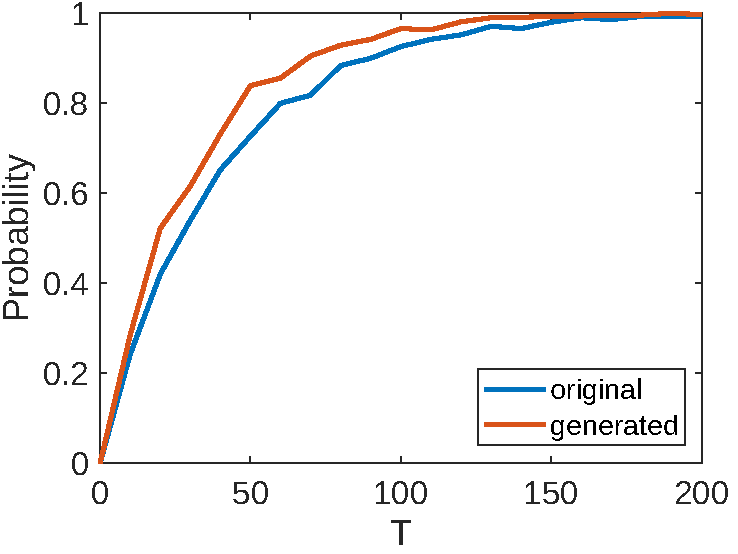
\includegraphics[scale=0.35]{example2.pdf}	
	\caption{Probability that a block is created within $T$ time units, $0\leq T\leq 200$}
	\label{ex5-res}
	\end{figure}
        The generated code is very similar the one outlined in
        \cite{DBLP:journals/distribledger/GallettaLMV23}, with the
        main distinction being the greater number of lines in our
        generated model.  This difference is due to the fact that
        certain commands could be combined, but our generation lacks
        the automatic capability to perform this check. While the
        results obtained for the probability of creating a block within the time $T$
        reported in Figure \ref{ex5-res} exhibit similarity, running
        simulations for the generated model takes PRISM 39.016
        seconds, compared to the 22.051 seconds required for the
        original model.



\mypar{Synchronous Leader Election.}
This case study examines the synchronous leader election protocol proposed by Itai $\&$ Rodeh~\cite{IR90}, designed to elect a leader in a ring of $N$ processors by exchanging messages. The protocol operates in rounds, where each processor selects a random ID from $\{1, \ldots, K\}$, circulates it around the ring, and determines if a unique maximum ID exists. If so, the processor with this ID becomes the leader; otherwise, the process repeats in the next round.

For illustration, we considered the case where $ N=4 $ and $ K=8 $, following the PRISM model\footnote{\url{https://www.prismmodelchecker.org/casestudies/synchronous_leader.php}}. We modeled this example in our choreographic language, as shown in Listing~\ref{leader-code}, capturing the protocol's behavior and dynamics.

\begin{lstlisting}[style=chor-color,caption={Choreography for the Synchronous Leader Election Protocol.},captionpos=b,label={leader-code}]
   {
   Election := 
      allSynch{ j in [1...4]
         Process[j] : (true -> "1/K" : "(p[i]'=0)&(v[i]'=0)&(u[i]'=true)" 
                                 + $\ldots$ + "1/K" : "(p[i]'=0)&(v[i]'=7)&(u[i]'=true)") }.
      allSynch{
         Counter : ("(c<N-1)" -> "1" : "(c'=c+1)")
         Counter : ("(c=N-1)" -> "1" : "(c'=c)")
         Process1 : ("u1&!(p1=2)&(c<N-1)" -> "1" : "(u1'=true)&(v1'=v2)")
         Process1 : ("u1&(p1=2)&(c<N-1)" -> "1" : "(u1'=false)&(v1'=v2)&(p1'=0)")
         Process1 : ("!u1&(c<N-1)" -> "1" : "(u1'=false)&(v1'=v2)")
         Process1 : ("u1&!(p1=v2)&(c=N-1)" -> "1" : "(u1'=true)&(v1'=0)&(p1'=0)")
         Process1 : ("u1&(p1=v2)&(c=N-1)" -> "1" : "(u1'=false)&(v1'=0)&(p1'=0)")
         Process1 : ("!u1&(c=N-1)" -> "1" : "(u1'=false)&(v1'=0)")
         $\ldots$
      }.
      if "u1 | u2 | u3 | u4"@Counter then {
         Counter -> Process[i] : (["1*1"] "(c'=c)" "(u[i]'=false)&(v[i]'=0)&(p[i]'=0)". 
         allSynch {
            Counter : (true -> "1" : "(c'=c)")
            Process1 : (true -> "1" : " ")
            $\ldots$               
         } . END)
      }
      else{
         Counter -> Process[i] : (["1*1"] "(c'=1)" "(u[i]'=false)&(v[i]'=0)&(p[i]'=0)"  . Election)
      }      
   }
   \end{lstlisting} 
   While the generated model (Listing \ref{leader-prism}) successfully replicates the functionality of 
   the PRISM repository model, a key difference lies in the modular 
   structure of the two representations. 
   Specifically, the generated model adopts a simplified modular design by 
   grouping transitions more compactly in certain modules, such as the \codeprism{Counter} module. 
   This simplification reduces redundancy and may improve readability without altering the correctness or outcomes of the protocol. Importantly, this structural refinement does not impact the behavior of the system, as the generated model remains functionally equivalent to the original PRISM repository model, as displayed in Figure \ref{leader-res}.

   \begin{lstlisting}[style=prism-color,caption={Generated PRISM program},captionpos=b,label={leader-prism}]
   module Counter
      Counter : [0..4] init 0;
      c : [0..N-1] init 0;
      [YQBDX] (Counter = 0)&(c<N-1) -> 1 : (c'=c+1)&(Counter'=1);
      [YQBDX] (Counter = 0)&(c=N-1) -> 1 : (c'=c)&(Counter'=1);
      [ELTMI] (Counter=1)&(u1 | u2 | u3 | u4) -> 1 : (c'=c)&(Counter'=2);
      [LJTIP] (Counter=1)&!(u1 | u2 | u3 | u4) -> 1 : (c'=1)&(Counter'=0);
      [AWUQP] (Counter = 2)-> 1 : (c'=c)&(Counter'=2);
   endmodule
   module Process1
   Process1 : [0..4] init 0;
      p1 : [0..K-1] init 0;
      v1 : [0..K-1] init 0;
      u1 : bool;
      [BKKXT](Process1 = 0) ->  1/K:(p1'=0)&(v1'=0)&(u1'=true)&(Process1'=1) 
                                 + 1/K:(p1'=1)&(v1'=1)&(u1'=true)&(Process1'=1) 
                                 + 1/K:(p1'=2)&(v1'=2)&(u1'=true)&(Process1'=1) 
                                 + 1/K:(p1'=2)&(v1'=3)&(u1'=true)&(Process1'=1) 
                                 + 1/K:(p1'=2)&(v1'=4)&(u1'=true)&(Process1'=1) 
                                 + 1/K:(p1'=2)&(v1'=5)&(u1'=true)&(Process1'=1) 
                                 + 1/K:(p1'=2)&(v1'=6)&(u1'=true)&(Process1'=1) 
                                 + 1/K:(p1'=2)&(v1'=7)&(u1'=true)&(Process1'=1);
      [YQBDX] (Process1 = 1)&u1&!(p1=2)&(c<N-1) -> 1 : (u1'=true)&(v1'=v2)&(Process1'=2);
      [YQBDX] (Process1 = 1)&u1&(p1=2)&(c<N-1) -> 1 : (u1'=false)&(v1'=v2)&(p1'=0)&(Process1'=2);
      [YQBDX] (Process1 = 1)&!u1&(c<N-1) -> 1 : (u1'=false)&(v1'=v2)&(Process1'=2);
      [YQBDX] (Process1 = 1)&u1&!(p1=v2)&(c=N-1) -> 1 : (u1'=true)&(v1'=0)&(p1'=0)&(Process1'=2);
      [YQBDX] (Process1 = 1)&u1&(p1=v2)&(c=N-1) -> 1 : (u1'=false)&(v1'=0)&(p1'=0)&(Process1'=2);
      [YQBDX] (Process1 = 1)&!u1&(c=N-1) -> 1 : (u1'=false)&(v1'=0)&(Process1'=2);
      [ELTMI] (Process1=2) -> 1 : (u1'=false)&(v1'=0)&(p1'=0)&(Process1'=3);
      [LJTIP] (Process1=2) -> 1 : (u1'=false)&(v1'=0)&(p1'=0)&(Process1'=0);
      [AWUQP] (Process1 = 3) -> 1 :  (Process1'=4);
   endmodule
   $\ldots$
   \end{lstlisting}


   \begin{figure}[h]
      \centering
      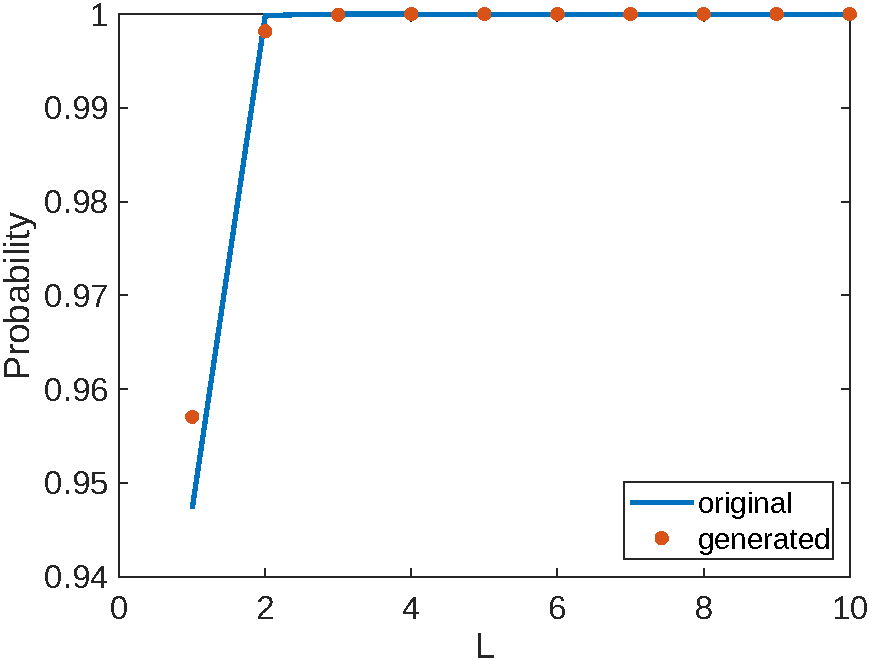
\includegraphics[scale=0.35]{leader.pdf}	
      \caption{The probability of electing a leader within $L$ rounds, with $1 \leq L \leq 10$}
      \label{leader-res}
      \end{figure}
\begin{comment}
\subsection{Problems}
\label{sec:problems}
While testing our choreographic language, we noticed that some of the case studies presented in the 
PRISM documentation \cite{PRISMdoc} cannot be modeled by using our language.
The reasons are various, in this section we try to outline the problems.

\begin{itemize}
\item \textbf{Asynchronous Leader Election}\footnote{\url{https://www.prismmodelchecker.org/casestudies/asynchronous_leader.php}}:
 processes synchronize with the same label but the conditions are different.
 We include in our language the \texttt{it-then-else} statement but we do not allow 
 the \texttt{if-then} (without the \texttt{else}). This is done because in this way, we do not 
 incur in deadlock states.
\item  \textbf{Probabilistic Broadcast Protocols}\footnote{\url{https://www.prismmodelchecker.org/casestudies/prob_broadcast.php}}:
 also in this case, the problem are the labels of the synchronizations.
 In fact, all the processes synchornize with the same label on every actions.
 This is not possible in our language, since a label is unique for every synchronization between two (or more) processes.
\item \textbf{Cyclic Server Polling System}\footnote{\url{https://www.prismmodelchecker.org/casestudies/polling.php}}:
 in this model, the processes \texttt{station$_i$} do two different things in the same state.
 More precicely, at the state 0 (\texttt{s$_i$=0}), the processes may synchornize with the process
 \texttt{server} or may change their state without any synchronization.
 In out language, this cannot be formalized since the synchronization is a branch action,
 so there should be another option with a synchronization.


\end{itemize}
\end{comment}




\mypar{Dining Cryptographers}
The generated model for this example does not faithfully model the original one. We chose 
to include it in the paper to demonstrate the limitations of our approach, 
specifically in cases where the abstraction may not fully capture the behavior of the original protocol. 
This allows us to analyze and understand where discrepancies may arise, 
highlighting areas for improvement in the model generation process.
This case study explores the dining cryptographers protocol introduced by Chaum~\cite{Cha88}, which allows a group of $N$ cryptographers to determine whether their master has anonymously paid for dinner without revealing the identity of the payer. The protocol functions by having each cryptographer flip a fair coin and share the outcome with their right-hand neighbor. Each cryptographer then publicly declares whether the two coins they observe—one they flipped and one received from the left—match or differ. If a cryptographer is the payer, they deliberately alter their response. The final count of "agree" statements follows a predictable pattern: for an odd number of cryptographers, an odd count indicates that one of them paid, while an even count means the master paid. This pattern reverses for an even number of participants.

To illustrate the protocol, we examined the case where $N=3$, using the PRISM model\footnote{\url{https://www.prismmodelchecker.org/casestudies/dining_cryptographers.php}} reported in the official repository. We expressed this scenario in our choreographic language, as shown in Listing~\ref{dc-code}.
\begin{lstlisting}[style=chor-color,caption={Choreography for the Dining Cryptographers Protocol.},captionpos=b,label={dc-code}]
{
   Crypto := if "(coin[i]=0)"@crypt[i] then {
                  crypt[i] -> crypt[i] : (+["0.5*1"] "(coin[i]'=1)" . Crypto2
                                             +["0.5*1"] "(coin[i]'=2)" . Crypto2) 
               }
               else{ Crypto }

   Crypto2 := if "((coin[i]>0)&(coin[i+1]>0))"@crypt[i] then{
                  if "(coin[i]=coin[i+1])"@crypt[i] then {
                     if "(pay=p[i])"@crypt[i] then { Crypto3 }
                     else{ ["1"] "(agree[i]'=1)"@crypt[i]. Crypto3 }
                  }
                  else{
                        if "(pay=p[i])"@crypt[i] then { ["1"] "(agree[i]'=1)"@crypt[i]. Crypto3 }
                        else{ Crypto3 }
                  }
               }
               else { Crypto2 }

   Crypto3 := allSynch{ j in [1...3]
                  crypt[j] : (true -> "1" : "true;" )
               }.END
}
\end{lstlisting}
This code defines a choreography model using three distinct choreographies (\texttt{Crypto}, \texttt{Crypto2}, and \texttt{Crypto3}) to avoid redundancy and optimize the code structure. By using separate choreographies, we can reuse common logic without rewriting the entire code.
The initial probabilistic branching demonstrates the use of recursion, where both branches of the probabilistic transition ultimately lead to the same state. 

In fact, in the generated PRISM model in Listing~\ref{dc-code-prism}, we can observe that from the initial state \codeprism{crypt1 = 0}, we transition to two possible branches where \codeprism{crypt1 = 1} regardless of whether coin1 takes the value 1 or 2. This is a result of the recursion in the choreography, where both branches follow the same recursive path that leads to \codeprism{crypt1 = 1}. The transitions in the model are shown in the following PRISM code, where both transitions have a 50$\%$ probability of either setting \codeprism{coin1 = 1} or \codeprism{coin1 = 2}, and both lead to the same updated state \codeprism{crypt1 = 1}. Note that the code provided here only shows a part of the generated PRISM model. The code for \codeprism{crypt2} and \codeprism{crypt3} follows the same structure.

\begin{lstlisting}[style=prism-color,caption={Generated PRISM program},captionpos=b,label={dc-code-prism},escapechar=|]
   $\ldots$
   module crypt1
   crypt1 : [0..2] init 0;
   coin1 : [0..2] init 0;
   s1 : [0..1] init 0;
   agree1 : [0..1] init 0;
   [] (crypt1=0)&((coin1=0)) -> 0.5 : (coin1'=1)&(crypt1'=1)+0.5 : (coin1'=2)&(crypt1'=1); |\label{first-line-crypto}|
   [] (crypt1=0)&!((coin1=0)) -> 1:(crypt1'=0);
   [] (crypt1=1)&(coin1>0)&(coin2>0)&((coin1=coin2))&!((pay=p1)) -> 1:(agree1'=1)&(crypt1'=2);
   [] (crypt1=1)&(coin1>0)&(coin2>0)&((coin1=coin2))&((pay=p1)) -> 1:(crypt1'=2);
   [] (crypt1=1)&(coin1>0)&(coin2>0)&!((coin1=coin2))&((pay=p1)) -> 1:(agree1'=1)&(crypt1'=2);
   [] (crypt1=1)&(coin1>0)&(coin2>0)&!((coin1=coin2))&!((pay=p1))-> 1:(crypt1'=2);
   [LERZX] (crypt1 = 2) -> 1:(crypt1'=2);
   endmodule
   $\ldots$
\end{lstlisting}

In this case, however, the generated model does not exhibit the same behavior as the original one in the PRISM repository. When analyzing the probability of anonimity, the result obtained by the original model, as reported on the website, is 0.25, whereas in our generated model, the probability is 0. This discrepancy arises from a fundamental difference in how the initial state is handled between the two models.

In the original PRISM model, the transition is defined as:
\begin{lstlisting}[style=prism-color, frame=none, numbers=none]
   [] (coin1=0) -> 0.5 : (coin1'=1)&(crypt1'=1) + 0.5 : (coin1'=2)&(crypt1'=1);
   \end{lstlisting}
Here, the transition occurs from \codeprism{coin1 = 0} to \codeprism{coin1 = 1} or \codeprism{coin1 = 2}, without any dependency on the \codeprism{crypt1} state. This allows for a transition regardless of the initial value of \codeprism{crypt1}.
In contrast, in our generated model, the transition is conditional on both \codeprism{coin1 = 0} and \codeprism{crypt1 = 0}, as shown at line \ref{first-line-crypto} of Listing \ref{dc-code-prism}.
As a result, the model can only transition when both conditions are met, but in the original model, such a restriction does not exist. This difference in the initial state setup explains why the probability of certain events and the number of states and transtitions in our generated model differ significantly from that of the original model (95 states and 194 transitions in our model vs. 380 and 776 in the original model).

%%% Local Variables: 
%%% mode: latex
%%% TeX-master: "main"
%%% End: